% !TEX TS-program = xelatex
% !TEX encoding = UTF-8

% XeLaTeX Memo Version 2
% Author:  Tanimodori (Tanimodoli@gmail.com)
% License: MIT License

% == 文档选项 ==
\documentclass[12pt]{article}

% == XeTeX 选项 ==
% 针对中文自动换行
\XeTeXlinebreaklocale "zh" %
% 字与字之间加入0pt至1pt的间距,确保左右对齐
\XeTeXlinebreakskip = 0pt plus 1pt %

% == 版式 ==
% 页边距
\usepackage{geometry}
\geometry{left=1.5cm,right=1.5cm,top=1.5cm,bottom=2cm,a4paper}
% 行首缩进2字符
\usepackage{indentfirst}
\setlength{\parindent}{2em}
% 1.5倍行距
\usepackage{setspace}
\onehalfspacing
% 跨页表格
\usepackage{longtable}
% 多行
\usepackage{multirow}
% 固定float位置
\usepackage{float}

% == 字体 ==
\usepackage{xeCJK,fontspec}
% 设置英文宋体、黑体、等宽字体
\setmainfont[AutoFakeSlant=0.2]{Source Han Serif SC}
\setsansfont[AutoFakeSlant=0.2]{Source Han Sans SC}
\setmonofont{Sarasa Mono SC}
% 设置中文宋体、黑体、等宽字体
\setCJKmainfont[AutoFakeSlant=0.2]{Source Han Serif SC}
\setCJKsansfont[AutoFakeSlant=0.2]{Source Han Sans SC}
\setCJKmonofont{Sarasa Mono SC}
% 使用更大的\textbullet
\renewcommand{\labelitemi}{\raisebox{0.1em}{$\bullet$}}

% == 图形、颜色 ==
\usepackage{metalogo}
\usepackage{graphicx}
\usepackage[svgnames]{xcolor}
\definecolor{colorTeX}{RGB}{0,0,0}
\definecolor{colorLaTeX}{RGB}{0,128,128}
\definecolor{colorPKG}{RGB}{131,80,99}
\definecolor{colorMACRO}{RGB}{0,172,233}
\usepackage{tikz}
\usetikzlibrary{arrows,arrows.meta,calc,graphs,quotes}
\usetikzlibrary{shapes,shapes.gates.logic.US,shapes.gates.logic.IEC}
\usepackage[american,RPvoltages]{circuitikz}
% 卡诺图
\usepackage{karnaugh-map}
% 流程图
\usepackage{flowchart}

\tikzset{
    tag/.style args={#1}{fill=#1, text=white, rounded rectangle, minimum height=0.8cm}
}

\DeclareRobustCommand{\tagTeX}{\tikz[baseline=-0.8ex]{\node [tag=colorTeX]{\small\TeX};}\ }
\DeclareRobustCommand{\tagLaTeX}{\tikz[baseline=-0.8ex]{\node [tag=colorLaTeX]{\small\LaTeX};}\ }
\DeclareRobustCommand{\tagPKG}{\tikz[baseline=-0.8ex]{\node [tag=colorPKG]{\small PKG};}\ }
\DeclareRobustCommand{\tagMACRO}{\tikz[baseline=-0.8ex]{\node [tag=colorMACRO]{\small MACRO};}\ }

% == 数学符号 ==
\usepackage{amsmath,amssymb,amsthm}
\usepackage{unicode-math}

% == 代码 ==
\usepackage{listings}
\lstset{
    basicstyle=\small\ttfamily
}
% LaTeX 预设
\lstdefinestyle{customlatex}{
    language=[LaTeX]TeX,
    commentstyle=\color{Brown},
    keywordstyle=\color{Green}\bfseries,
    texcsstyle=*\color{blue}\bfseries,
    %directivestyle={\color{blue}\bfseries},
    numbers=none,
    keepspaces=true,
    columns=fixed,
    basewidth=0.5em,
    morekeywords={document, titlepage}
}
\lstdefinestyle{linewrap}{
    basicstyle=\footnotesize\ttfamily,
    breaklines=true,
    postbreak=\mbox{\textcolor{red}{$\hookrightarrow$}\space}
}
% Matlab
\usepackage{matlab-prettifier}

% == 源代码和结果展示 ==
\usepackage{showexpl}

% == 解析器 ==
\usepackage{xparse}


\title{Tanimodori的\ \LaTeX\ 备忘录 \\{\normalsize v 0.1.0}}
\author{Tanimodori}
\date{2020年7月10日} 

\begin{document}
\maketitle

\setcounter{section}{-1}
\section{约定}

\begin{itemize}
    \item \tagTeX  表示内容属于由Plain \TeX 
    \item \tagLaTeX  表示内容属于\LaTeX
    \item \tagPKG  表示内容属于宏包
    \item \tagMACRO  表示内容属于本文中的宏
\end{itemize}

\clearpage

\section{基本}

\subsection{\LaTeX 文档基本格式\ \tagLaTeX}

\begin{lstlisting}[frame=single,style=customlatex]
% !TEX TS-program = xelatex
% !TEX encoding = UTF-8
\XeTeXlinebreaklocale "zh"
\XeTeXlinebreakskip = 0pt plus 1pt     % 编译引擎选项、编码
\documentclass[12pt]{article}          % 全局选项、文档属性
\usepackage{xeCJK,fontspec}            % 宏包及其选项
\usepackage{graphicx}
\usepackage{amsmath,amssymb,amsthm}
\title{\LaTeX\ Test}                   % 标题
\author{\LaTeX\ User}                  % 作者
\date{yyyy.mm.dd}                      % 日期
\begin{document}                       % 导言区结束,进入正文
\maketitle
\section{Foo}                          % 节
\subsection{Bar}                       % 小节
The quick fox jumps over the lazy dog. % 正文
\end{document}                         % 正文结束
\end{lstlisting}

\subsection{空格\ \tagTeX\ \tagLaTeX}

一次 \LaTeX\ 源文件编译过程中的主要步骤包括:

\begin{enumerate}
    \item 前端编辑器(例如TeXWorks)根据源文件和用户设置交给对应的引擎(例如 \XeTeX\ )
    \item 引擎将源文件令牌化
    \item 引擎根据令牌序列输出结果。
\end{enumerate}

在令牌化过程中,单个空格、多个空格或者单个换行符会被看作一个空格令牌,多个换行符会被看做换行令牌。但是控制字\footnote{Control Word,由反斜杠和字母序列组成,例如“\texttt{\backslash LaTeX},是控制序列的一种。”}末尾的空格字符会被忽略,不会作为空格令牌。还需加上“\texttt{\backslash}\lstinline[showspaces=true]{ }”来插入一个控制空格。控制换行符可以通过“\texttt{\backslash\backslash}”插入

\begin{LTXexample}[style=customlatex]
\LaTeX       without space\\
\LaTeX\ with space!
\end{LTXexample}

我们用尺度\textit{(dimension)}一词来描述空格的长度。尺度由“实数+单位”构成,例如“\lstinline{5pt}”、“\lstinline{-1.1 em}”、“\lstinline{+,6cm}”都是合法的尺度。在\TeX 中,可以通过\lstinline!\hskip <dimen> !、\lstinline!\vskip <dimen> !插入水平和垂直空格。\LaTeX 的对应命令为\lstinline!\hspace{<dimen>}!和\lstinline!\vspace{<dimen>}!。一般来说,由于历史遗留问题,我们应尽量使用\LaTeX 包装好的命令,避免使用 \TeX 命令。

能够产生水平空格的常见指令见下表。

\begin{figure}[H]
    \centering
    \renewcommand{\arraystretch}{1.2}
    \begin{longtable}{|c|l|p{1.6cm}|l|p{1.6cm}|}
    \hline
    \multirow{2}*{空格宽度} & \multicolumn{2}{|c|}{文本模式} & \multicolumn{2}{|c|}{数学模式} \\\cline{2-5}
    ~ & 代码 & 示例 & 代码 & 示例 \\\hline\endhead
    \multirow{2}*{\shortstack{.16667em\\或3mu}} & \verb|a\,b|  & a\,b & \verb|$a\,b$| & $a\,b$ \\\cline{2-5}
    ~ & \verb|a\thinspace b| & a\thinspace b & \verb|$a\thinspace b$| & $a\thinspace b$ \\\hline
    \multirow{2}*{-3mu} & \multicolumn{2}{|c|}{\multirow{2}*{}} & \verb|$a\!b$| & $a\!b$ \\\cline{4-5}
    ~ & \multicolumn{2}{|c|}{} & \footnotesize\verb|$a\mkern-\thinmuskip b$| & $a\mkern-\thinmuskip b$ \\\hline
    \multirow{3}*{\footnotesize\shortstack{4.0mu\\ plus 2.0mu\\ minus 4.0mu}} & \multicolumn{2}{|c|}{\multirow{3}*{}} & \verb|$a\>b$| & $a\>b$ \\\cline{4-5}
    ~ & \multicolumn{2}{|c|}{} & \verb|$a\:b$|                  & $a\: b$ \\\cline{4-5}
    ~ & \multicolumn{2}{|c|}{} & \footnotesize\verb|$a\mkern\medmuskip b$|   & $a\mkern\medmuskip b$   \\\hline
    \multirow{2}*{\footnotesize\shortstack{5.0mu\\ plus 5.0mu}} & \multicolumn{2}{|c|}{\multirow{2}*{}} & \verb|$a\;b$| & $a\;b$ \\\cline{4-5}
    ~ & \multicolumn{2}{|c|}{} & \footnotesize\verb|$a\mkern\thickmuskip b$| & $a\mkern\thickmuskip b$ \\\hline
    .5em & \verb|a\enspace b| & a\enspace b & \verb|$a\enspace b$| & $a\enspace b$ \\\hline
    1em  & \verb|a\quad b|    & a\quad b    & \verb|$a\quad b$|    & $a\quad b$    \\\hline
    2em  & \verb|a\qquad b|   & a\qquad b   & \verb|$a\qquad b$|   & $a\qquad b$   \\\hline
    \multirow{3}*{<len>} & \verb|a\hskip 1em b| & a\hskip 1em b & \verb|$a\hskip 1em b$| & $a\hskip 1em b$ \\\cline{2-5}
    ~ & \verb|a\kern 1pc b|     & a\kern 1pc b     & \verb|$a\kern 1pc b$|     & $a\kern 1pc b$     \\\cline{2-5}
    ~ & \verb|a\hspace{25pt} b| & a\hspace{25pt} b & \verb|$a\hspace{25pt} b$| & $a\hspace{25pt} b$ \\\hline
    \multirow{2}*{<stuff>} & \verb|axyzb| & axyzb & \verb|$axyzb$| & $axyzb$ \\\cline{2-5}
    ~ & \verb|a\hphantom{xyz}b| &  a\hphantom{xyz}b & \verb|$a\hphantom{xyz}b$| &  $a\hphantom{xyz}b$ \\\hline
    \multirow{2}*{\footnotesize inter-word} & \verb|a{ }b| & a{ }b & \verb|$a{ }b$| & $a{ }b$ \\\cline{2-5}
    ~ & \verb|a\space b| &  a\space b & \verb|$a\space b$| &  $a\space b$ \\\hline
    \footnotesize control     & \verb|a\ b|      &  a\ b      & \verb|$a\ b$|      &  $a\ b$      \\\hline
    \footnotesize unbreakable & \verb|a~b|       &  a~b       & \verb|$a~b$|       &  $a~b$       \\\hline
    \multirow{2}*{\footnotesize rubber} &\verb|a\hfill b| &  a\hfill b & \verb|$a\hfill b$| &  $a\hfill b$ \\\cline{2-5}
    ~      & \verb|a\hspace{\fill} b| &  a\hspace{\fill} b & \verb|$a\hspace{\fill} b$| &  $a\hspace{\fill} b$ \\\hline
    \end{longtable}
\end{figure}

其中 \lstinline{mu} 是数学模式下的单位长度。 \lstinline{<dimen> plus <dimen> minus <dimen>} 除了定义空格的长度以外,还定义了空格的伸缩量。\lstinline{\hphantom}会提供与参数水平尺寸相同的空格。“\lstinline{~}”、\lstinline!\hspace*!和\lstinline!\vspace*!产生的空格是不换行空格,也就是说\LaTeX 不会在此处换行。\lstinline!\hfill!、\lstinline!\vfill!(\TeX)、\lstinline!\hspace{\fill}!、\lstinline!\vspace{\fill}!(\LaTeX)将产生填满剩余空间的空格,若有多个,则按照比例分配,例如:

\begin{LTXexample}[style=customlatex]
左对齐 \hspace*{\fill}\\
\hspace*{\fill} 右对齐\\
\hspace*{\fill} 居中 \hspace*{\fill}
\end{LTXexample}

\subsection{字体\ \tagLaTeX }

\subsubsection{指定字体}

我们首先需要导入\lstinline{xeCJK}和\lstinline{fontspec}宏包,然后才能指定中英文字体。

\begin{lstlisting}[frame=single,style=customlatex]
% 导言区
\usepackage{xeCJK,fontspec}
% 设置英文宋体、黑体、等宽字体
\setmainfont{Source Han Serif SC}
\setsansfont{Source Han Sans SC}
\setmonofont{Sarasa Mono SC}
% 设置中文宋体、黑体、等宽字体
\setCJKmainfont{Source Han Serif SC}
\setCJKsansfont{Source Han Sans SC}
\setCJKmonofont{Sarasa Mono SC}
\end{lstlisting}

我们还可以给字体指定伪斜体与伪粗体

\begin{lstlisting}[frame=single,style=customlatex]
\setmainfont[AutoFakeSlant=0.2, AutoFakeBold=1.5]{Source Han Serif SC}
\end{lstlisting}

\subsubsection{指定字形}

\begin{table}[H]
    \centering
    \begin{tabular}{|l|l|l|} \hline
    命令 & 等价命令 & 效果 \\\hline
    \verb|\textnormal{...}| & \verb|{\normalfont ...}| & {\normalfont sample text 示例文本} \\\hline
    \verb|\emph{...}|   & \verb|{\em ...}|       & {\em sample text 示例文本} \\\hline
    \verb|\textrm{...}| & \verb|{\rmfamily ...}| & {\rmfamily sample text 示例文本} \\\hline
    \verb|\textsf{...}| & \verb|{\sffamily ...}| & {\sffamily sample text 示例文本} \\\hline
    \verb|\texttt{...}| & \verb|{\ttfamily ...}| & {\ttfamily sample text 示例文本} \\\hline
    \verb|\textup{...}| & \verb|{\upshape ...}|  & {\upshape sample text 示例文本} \\\hline
    \verb|\textit{...}| & \verb|{\itshape ...}|  & {\itshape sample text 示例文本} \\\hline
    \verb|\textsl{...}| & \verb|{\slshape ...}|  & {\slshape sample text 示例文本} \\\hline
    \verb|\textsc{...}| & \verb|{\scshape ...}|  & 不支持 \\\hline
    \verb|\textbf{...}| & \verb|{\bfseries ...}| & {\bfseries sample text 示例文本} \\\hline
    \verb|\textmd{...}| & \verb|{\mdseries ...}| & {\mdseries sample text 示例文本} \\\hline
    \verb|\textlf{...}| & \verb|{\lfseries ...}| & 不支持 \\\hline
    \end{tabular}
\end{table}

\subsubsection{指定字体大小}

\begin{table}[H]
    \centering
    \begin{tabular}{|l|l|} \hline
    命令 & 效果 \\\hline
    \verb|\tiny|         &\tiny{sample text 示例文本}         \\\hline
    \verb|\scriptsize|   &\scriptsize{sample text 示例文本}   \\\hline
    \verb|\footnotesize| &\footnotesize{sample text 示例文本} \\\hline
    \verb|\small|        &\small{sample text 示例文本}        \\\hline
    \verb|\normalsize|   &\normalsize{sample text 示例文本}   \\\hline
    \verb|\large|        &\large{sample text 示例文本}        \\\hline
    \verb|\Large|        &\Large{sample text 示例文本}        \\\hline
    \verb|\LARGE|        &\LARGE{sample text 示例文本}        \\\hline
    \verb|\huge|         &\huge{sample text 示例文本}         \\\hline
    \verb|\Huge|         &\Huge{sample text 示例文本}         \\\hline
    \end{tabular}
\end{table}

\subsubsection{指定字体颜色\ \tagPKG}

\begin{LTXexample}[style=customlatex]
    \usepackage{xcolor} % 导言区
    {\color{red} red text}\\
    \textcolor{blue}{blue text}
\end{LTXexample}

\section{版式与结构}

\subsection{参考文献}

\begin{lstlisting}[style=customlatex, style=linewrap, frame=single]
\usepackage{hyperref}
\usepackage[hyperref=true,backend=biber,sorting=none,backref=false,doi=false,isbn=false,url=false]{biblatex}
\addbibresource{example.bib}
% 引言区
\begin{document}
Foo\parencite{Foo_Bar_2020}
\printbibliography[heading=none]
\end{document}
\end{lstlisting}

%\subsection{页边距}
%\subsection{日期}
%\subsection{分割线}
%\subsection{自定义封面}
%\subsection{目录}
%\subsubsection{带超链接的目录}
%\subsection{附录}

\section{数学模式\ \tagTeX\tagLaTeX}

\paragraph{下花括号}\hspace{1pt}

\begin{LTXexample}[style=customlatex]
\[1\underbrace{0\cdots0}_{\text{10 zeros}}\]
\end{LTXexample}

\paragraph{分类}\hspace{1pt}

\begin{LTXexample}[style=customlatex]
\[x=\begin{cases}
    1,&y=1\\
    2,&y=2\\
    0,&\text{otherwise}.
\end{cases}\]
\end{LTXexample}

\paragraph{矩阵}\hspace{1pt}

\begin{LTXexample}[style=customlatex]
\[A=\begin{bmatrix}
    1&2\\
    3&4
\end{bmatrix}\]
\end{LTXexample}

\paragraph{等式}\hspace{1pt}

\begin{LTXexample}[style=customlatex]
\begin{equation}
    T_{0}(k)=\frac{1}{2} T_{0}(k-1)
\end{equation}
\end{LTXexample}

\paragraph{连等式}\hspace{1pt}

\begin{LTXexample}[style=customlatex]
\[\begin{aligned}
y&=(x+1)(x-1)\\
&=x^2-1
\end{aligned}\]
\end{LTXexample}

%\section{图片}
%\subsection{位图、矢量图、PDF}
%长图,图表标题,自定义封面


%\subsection{列表}
\section{表格\ \tagLaTeX}

\paragraph{tabular}\hspace{1pt}

\begin{LTXexample}[style=customlatex]
\begin{center}
\begin{tabular}{|l|l|l|l|}
\hline
十进制数& 4-3-2-1编码 \\\hline
0      & 0000  \\\hline
1      & 0001  \\\hline
2      & 0010  \\\hline
3      & 0100  \\\hline
4      & 1000  \\\hline
5      & 1001  \\\hline
6      & 1010  \\\hline
7      & 1100  \\\hline
8      & 1101  \\\hline
9      & 1110  \\\hline
\end{tabular}
\end{center}
\end{LTXexample}

\paragraph{多行与多列}\tagPKG

\begin{LTXexample}[style=customlatex,style=linewrap]
\usepackage{multirow} %导言区
\begin{center}
\begin{tabular}{c|cc|c}\hline
    \multirow{2}*{现态}&\multicolumn{2}{|c|}{次态}&\multirow{2}*{当前输出}\\\cline{2-3}
    ~&$X=0$&$X=1$&~\\\hline
    a&c&c&1\\
    c&d&f&0\\
    d&f&a&1\\
    f&c&d&0\\\hline
\end{tabular}
\end{center}
\end{LTXexample}

\section{代码\ \tagPKG}

\paragraph{Matlab}\hspace{1pt}

\begin{LTXexample}[style=customlatex]
\usepackage{listings}
\usepackage{matlab-prettifier} % 导言区
\begin{lstlisting}[style=Matlab-editor]
function xbar=mymean(x)
    t=0;
    n=length(x);
    for i=1:n
        t=t+x(i);
    end
    xbar=t/n;
end
\end{lstlisting}
\end{LTXexample}

\paragraph{x86汇编}\hspace{1pt}

\begin{LTXexample}[varwidth,style=customlatex,style=linewrap]
\usepackage{listings} % 导言区
\lstdefinestyle{customasm}{
language=[x86masm]Assembler,
basicstyle=\linespread{1.0}\small\ttfamily,
commentstyle=\color{Brown},
keywordstyle=\color{blue}\bfseries,
stringstyle=\color{Green}\bfseries,
keepspaces=true,
columns=fixed,
basewidth=0.5em,
}
\lstinputlisting[style=customasm]{x86asm_example.asm}
\end{LTXexample}

\paragraph{C}\hspace{1pt}

\begin{LTXexample}[varwidth,style=customlatex,style=linewrap]
\usepackage{listings} % 导言区
\lstdefinestyle{customc}{
language=C,%
keepspaces=true,%
columns=fixed,%
basewidth=0.5em,%
basicstyle=\ttfamily,%
breaklines=true,%
commentstyle=\color{Green},%
keywordstyle=\color{blue}\bfseries,%
stringstyle=\color{Brown}\bfseries,%
numberstyle=\ttfamily\color{Gray},%
showstringspaces=false%
}
\lstinputlisting[style=customc]{c_example.c}
\end{LTXexample}
    

\paragraph{Python}\hspace{1pt}


\begin{LTXexample}[style=customlatex,style=linewrap]
\usepackage{listings} % 导言区
\lstdefinestyle{custompython}{
    language=Python,
    keepspaces=true,
    columns=fixed,
    basewidth=0.5em,
    basicstyle=\ttfamily,
    breaklines=true,
    commentstyle=\color{Green},
    keywordstyle=\color{blue}\bfseries,
    stringstyle=\color{Brown}\bfseries,
    showstringspaces=false
}
\lstinputlisting[style=custompython]{python_example.py}
\end{LTXexample}

\paragraph{diff}\hspace{1pt}

\begin{LTXexample}[style=customlatex,style=linewrap]
\usepackage{xcolor}
\definecolor{diffstart}{named}{gray}
\definecolor{diffincl}{named}{Green}
\definecolor{diffrem}{named}{Red}
\usepackage{listings} 
\lstdefinestyle{customdiff}{
    language=C,
    keepspaces=true,
    columns=fixed,
    basewidth=0.5em,
    basicstyle=\ttfamily,
    breaklines=true,
    commentstyle=\color{Green},
    keywordstyle=\color{blue}\bfseries,
    stringstyle=\color{Brown}\bfseries,
    numberstyle=\ttfamily\color{Gray},
    showstringspaces=false,
    morecomment=[f][\color{diffstart}]{@@},
    morecomment=[f][\color{diffincl}]{+\ },
    morecomment=[f][\color{diffrem}]{-\ },
    numbers=left,
    stepnumber=1
}
% LISTINGS linenumber hack
\makeatletter
\let\orig@lstnumber=\thelstnumber
\newcommand\lstsetnumber[1]{\gdef\thelstnumber{#1}}
\newcommand\lstresetnumber{\global\let\thelstnumber=\orig@lstnumber}
\makeatother
% 导言区
\begin{lstlisting}[style=customdiff,firstnumber=12, mathescape=true]
-   int i;
-   for (i = 0; i < N; i++)
-       pthread_create(&tid[i], NULL, thread, &i);$\lstresetnumber\setcounter{lstnumber}{11}$
+   int i, args[N];
+   for (i = 0; i < N; i++) {
+       args[i] = i;
+       pthread_create(&tid[i], NULL, thread, args + i);
+   }
\end{lstlisting} 
\end{LTXexample}


%\subsection{预设环境}


\section{Tikz\ \tagPKG}

\subsection{命令示例}

\paragraph{\texttt{\backslash foreach}}\hspace{1pt}

\begin{LTXexample}[pos=t, style=customlatex]
\begin{center}
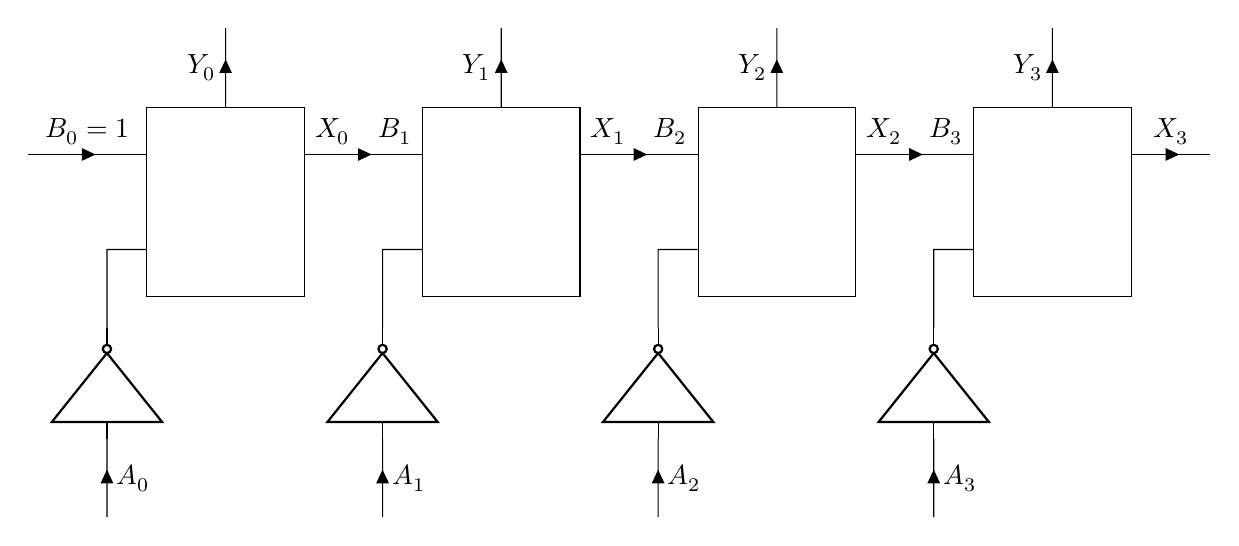
\begin{tikzpicture}[>=latex] 
\foreach \x in {1, 2, 3, 4} {
    \pgfmathtruncatemacro{\xminus}{\x-1}
    \draw
    (\xminus*3.5,0) node[draw,minimum width=2cm,minimum height=2.4cm] (ha\x) {半加器}
    ($(ha\x.west)!0.5!(ha\x.south west)$) coordinate (ha\x-a)
    ($(ha\x.west)!0.5!(ha\x.north west)$) coordinate (ha\x-b)
    ($(ha\x.east)!0.5!(ha\x.north east)$) coordinate (ha\x-x)
    ($(ha\x.north)$) coordinate (ha\x-y)
    (ha\x-a) -| ++ (-0.5,-1) node[not port, anchor=out, rotate=90] (ha\x-an) {}
    (ha\x-an.in) to[short,i^<=${A_\xminus}$] ++ (0,-1)
    (ha\x-y) to[short,i^>=${Y_\xminus}$] ++ (0,1);
}
\foreach \x in {1, 2, 3} {
    \pgfmathtruncatemacro{\xminus}{\x-1}
    \pgfmathtruncatemacro{\xplus}{\x+1}
    \draw
    (ha\x-x) to[short,i^>=${X_\xminus\quad B_\x}$] (ha\xplus-b);
}
\draw
(ha1-b) to[short,i_<=${B_0=1}$] ++ (-1.5,0)
(ha4-x) to[short,i^>=${X_3}$] ++ (1,0);
\end{tikzpicture}
\end{center}
\end{LTXexample}

\subsection{内容示例}

\subsubsection{数字逻辑设计}

\paragraph{开关电路}\hspace{1pt}

\begin{LTXexample}[pos=t, style=customlatex]
\usepackage{tikz}
\usetikzlibrary{arrows,shapes}
\usepackage[american,RPvoltages]{circuitikz}
% 导言区
\begin{center}
\begin{circuitikz}[>=latex] 
\draw
(0,0) to [short,o-*] (1,0) coordinate (left_in) --++ (0,1) 
--++ (1,0) to[nos,->,l=$X$] ++ (0.5,0) --++ (1,0) 
--++ (0,-1) coordinate (left_out) to [short,*-*] ++ (1,0) coordinate (right_start)

(left_in) --++ (0,-1) 
--++ (1,0) to[nos,->,l=$Y$] ++ (0.5,0) --++ (1,0) 
-- (left_out)

(right_start) --++ (0,1) 
--++ (1,0) to[nos,->,l=$X$] ++ (0.5,0) --++ (1,0) 
--++ (0,-1) coordinate (right_end) to [short,*-o] ++ (1,0) coordinate(end)

(right_start) --++ (0,-1) 
--++ (1,0) to[nos,->,l=$Z$] ++ (0.5,0) --++ (1,0) 
-- (right_end);
\end{circuitikz}
\end{center}
\end{LTXexample}

\paragraph{门电路} \tagMACRO

首先导入 \texttt{xparse} 宏包

\begin{lstlisting}[frame=single,style=customlatex]
\usepackage{xparse} % 导言区
\end{lstlisting}

% \gatelabel

\makeatletter
\newcommand*{\gatelabel@unstarred}[2]{
\foreach \label [count=\li] in #2 {
    \draw (#1.input \li) ++ (-0.5,0) node (#1_i_\li) [left] {\label} -- (#1.input \li);
}
}
\newcommand*{\gatelabel@starred}[2]{
    \draw (#1.output) -- ++(0.5,0) node (#1_o) [right] {#2};
}
\newcommand*{\gatelabel}{\@ifstar{\gatelabel@starred}{\gatelabel@unstarred}}
\makeatother

% \fixname from https://tex.stackexchange.com/a/213815/220363
\tikzset{
    keep name/.style={prefix after command={\pgfextra{\let\fixname\tikzlastnode}}},
    pics/input labels/.initial={},
    pics/output label/.initial={},
    pics/select labels/.initial={},
    with input labels/.pic={
        \edef\ilabels{\pgfkeysvalueof{/tikz/pics/input labels}}%
        \foreach \ilabel [count=\li] in \ilabels {
            \draw (\fixname.input \li) ++ (-0.5,0) node (\fixname_i_\li) [left] {\ilabel} -- (\fixname.input \li);
        }
    },
    with input labels/.style={
        keep name,
        append after command = {
            pic {input labels={#1}, with input labels}
        }
    },
    with output label/.pic={
        \edef\olabel{\pgfkeysvalueof{/tikz/pics/output label}}%
        \draw (\fixname.output) -- ++(0.5,0) node (\fixname_o) [right] {\olabel};
    },
    with output label/.style={
        keep name,
        append after command = {
            pic {output label={#1}, with output label}
        }
    },
    with select labels/.pic={
        \edef\slabels{\pgfkeysvalueof{/tikz/pics/select labels}}%
        \foreach \slabel [count=\li] in \slabels {%
            \draw let \p1=(\fixname.bottom right corner),\p2=(\fixname.select \li) in (\p2) -- (\x2,\y1-10) node[below] {\slabel};%
        };
    },
    with select labels/.style={
        keep name,
        append after command = {
            pic {select labels={#1}, with select labels}
        }
    }
}

\texttt{\bfseries\string\gatelabel} 命令可以为门电路标记输入输出,其用法如下:

\begin{lstlisting}[escapechar=\%, frame=single, columns=flexible]
\gatelabel{}
\gatelabel*
\end{lstlisting}

注意:该命令只能处理输入在左侧,输出在右侧的门。使用示例如下。

\begin{LTXexample}[varwidth, style=customlatex, style=linewrap]
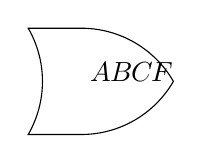
\begin{tikzpicture}
\node (or) [or gate US, draw, logic gate inputs=nnn,scale=2] {};
\gatelabel{or}{{$A$,$B$,$C$}}
\gatelabel*{or}{$F$}
\end{tikzpicture}
\end{LTXexample}

该命令的定义如下:

\lstinputlisting[frame=single,style=customlatex]{gatelabel.tex}

% \gatelink

\newcommand*\gatelink[3][0]{
\draw let \p1=(#2),\p2=(#3),\n1={\x1*0.5+\x2*0.5}
    in (\x1,\y1) -- ($(\n1,\y1)+(#1,0)$) |- (\x2,\y2);
}

\texttt{\bfseries\string\gatelink} 命令可以为连接两个门之间的输入输出,其用法如下

\begin{lstlisting}[escapechar=\%, frame=single, columns=flexible]
\gatelink[%\textit{offset}%]
\end{lstlisting}

注意:该命令只能处理输入在左侧,输出在右侧的门。使用示例如下。

\begin{LTXexample}[varwidth, style=customlatex, style=linewrap]
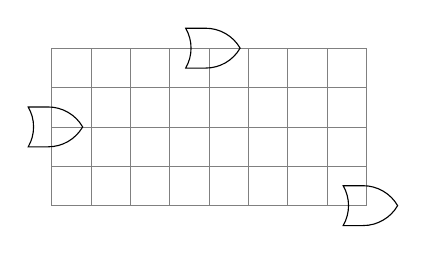
\begin{tikzpicture}[every node/.style={or gate US, draw}]
\draw[help lines, step=0.5cm] (0,0) grid (4,2);
\node (or1) at (0,1) {};
\node (or2) at (2,2) {};
\node (or3) at (4,0) {};
\gatelink{or1.output}{or2.input 1}
\gatelink[0.5]{or2.output}{or3.input 1}
\gatelink[-0.5]{or1.output}{or3.input 2}
\end{tikzpicture}
\end{LTXexample}
    
该命令的定义如下:

\lstinputlisting[frame=single,style=customlatex]{gatelink.tex}

使用以上两个命令的基本门电路用例如下:

\begin{LTXexample}[pos=t, style=customlatex, style=linewrap]
\usepackage{tikz}
\usetikzlibrary{arrows,shapes,shapes.gates.logic.US,shapes.gates.logic.IEC}
% 导言区
\begin{center}
\begin{tikzpicture}[>=latex]
\node (or) [or gate US, draw, logic gate inputs=nnnn,scale=2] at (4,-5) {};
\gatelabel*{or}{$F$}
\foreach \i/\list/\offset in 
{1/{$A$,$B$,$C'$}/0.5,2/{$A$,$C$,$D$}/-0.5,3/{$A'$,$B'$,$C$}/-0.5,4/{$A'$,$C'$,$D$}/0.5}
{
\node (and\i) [and gate US, draw, logic gate inputs=nnn, scale=2] at (0,-\i*2) {};
\gatelabel{and\i}{\list}
\gatelink[\offset]{and\i.output}{or.input \i}
}
\end{tikzpicture}
\end{center}
\end{LTXexample}


\paragraph{MUX} \tagMACRO

% mux & gateselectlabel
% see https://stackoverflow.com/questions/61729168/
\pgfkeys{
    /tikz/mux ports/.initial=1
}

\makeatletter
\pgfdeclareshape{muxshape}{
\inheritsavedanchors[from=trapezium] 
\inheritanchorborder[from=trapezium]
\inheritbackgroundpath[from=trapezium]
\foreach \anchor in {bottom left corner, top right corner, top left corner, bottom right corner, bottom side, left side, right side, top side, center, text, mid, base, mid west, base west, mid east, base east, west, east, north, south, north west, north east, south west, south east}{ \inheritanchor[from=trapezium]{\anchor} }
\savedmacro\numports{%
    \edef\numports{\pgfkeysvalueof{/tikz/mux ports}}%
}
\savedmacro\numselports{%
    \pgfmathtruncatemacro{\selports}{ceil(log2(\pgfkeysvalueof{/tikz/mux ports}))}
    \edef\numselports{\selports}%
}
\anchor{output}{\csname pgf@anchor@muxshape@top side\endcsname}
% input ports and select ports
\pgfutil@g@addto@macro\pgf@sh@s@muxshape{%
    % input ports
    \c@pgf@counta\numports\relax%
    \pgfmathloop%\
    \ifnum\pgfmathcounter>\c@pgf@counta%
    \else%
    \expandafter\xdef\csname pgf@anchor@muxshape@input\space\pgfmathcounter\endcsname{%
        \noexpand\pgf@sh@@muxshapeinputanchor{\pgfmathcounter}%
    }
    \repeatpgfmathloop%
    % select ports
    \c@pgf@counta\numselports\relax
    \pgfmathloop%\
    \ifnum\pgfmathcounter>\c@pgf@counta%
    \else%
    \expandafter\xdef\csname pgf@anchor@muxshape@select\space\pgfmathcounter\endcsname{%
        \noexpand\pgf@sh@@muxshapeselectanchor{\pgfmathcounter}%
    }
    \repeatpgfmathloop%
}
}

\def\pgf@sh@@muxshapeinputanchor#1{%
    \installtrapeziumparameters
    \lowerleftpoint
    \pgf@xa=\pgf@x \pgf@ya=\pgf@y
    \lowerrightpoint
    \pgf@xb=\pgf@x \pgf@yb=\pgf@y
    \pgfmathsetlength{\pgf@x}{\pgf@xa+(\pgf@xb-\pgf@xa)*#1/(\numports+1)}%
    \pgfmathsetlength{\pgf@y}{\pgf@ya+(\pgf@yb-\pgf@ya)*#1/(\numports+1)}%
}

\def\pgf@sh@@muxshapeselectanchor#1{%
    \installtrapeziumparameters
    \lowerrightpoint
    \pgf@xa=\pgf@x \pgf@ya=\pgf@y
    \upperrightpoint
    \pgf@xb=\pgf@x \pgf@yb=\pgf@y
    \pgfmathsetlength{\pgf@x}{\pgf@xa+(\pgf@xb-\pgf@xa)*#1/(\numselports+1)}%
    \pgfmathsetlength{\pgf@y}{\pgf@ya+(\pgf@yb-\pgf@ya)*#1/(\numselports+1)}%
}

\tikzset{
mux/.code={
    \pgfmathtruncatemacro{\si}{ceil(log2(#1))}%
    \pgfkeys{/tikz/mux ports=#1}
    \pgfkeys{
        /tikz/shape=muxshape,
        /tikz/draw,
        /tikz/trapezium stretches,
        /tikz/shape border rotate = 270,
        /tikz/minimum height=(\si+1)*0.4cm,
        /tikz/minimum width=\si*1.6cm
    }
}
}
\newcommand*\gateselectlabel[2]{%
\foreach \label [count=\ni] in #2 {%
    \draw let \p1=(#1.bottom right corner),\p2=(#1.select \ni) in (\p2) -- (\x2,\y1-10) node[below] {\label};%
};
}

\texttt{\bfseries mux} 样式的用法如下

\begin{lstlisting}[escapechar=\%, frame=single, columns=flexible]
\node [mux=%\textit{in-ports-numbers}%] {};
\end{lstlisting}

\texttt{\bfseries\string\gateselectlabel} 命令为门电路标记选择端口,其用法如下:

\begin{lstlisting}[escapechar=\%, frame=single, columns=flexible]
\gateselectlabel{}
\end{lstlisting}

示例代码如下

\begin{LTXexample}[pos=t,style=customlatex,style=linewrap]
\begin{center}
\begin{tikzpicture}
\node (mux) [mux=8] {};
\gatelabel{mux}{{$A$,$B$,$C$,$D$,$E$,$F$,$G$,$H$}}
\gatelabel*{mux}{$X$}
\gateselectlabel{mux}{{$P$,$Q$,$R$}}
\end{tikzpicture}
\end{center}
\end{LTXexample}

\texttt{mux} 样式的定义如下

\lstinputlisting[frame=single,style=customlatex,style=linewrap]{mux.tex}

\texttt{\string\gateselectlabel} 命令的定义如下

\lstinputlisting[frame=single,style=customlatex,style=linewrap]{gateselectlabel.tex}


\paragraph{线网图} \tagMACRO

\texttt{\bfseries paramlines}环境可以用于绘制线网图,其定义和示例如下:

\newcounter{pl@@netcount}
\newcounter{pl@@linecount}[pl@@netcount]
\NewDocumentEnvironment{paramlines}{O{5} O{1}}{%
    \stepcounter{pl@@netcount}%
    \newcommand\plparamdef[1]{%%
        \expandafter\edef\csname pl@##1\endcsname{\arabic{pl@@linecount}}%%
        \stepcounter{pl@@linecount}%%
    }
    \newcommand\plsetbasex[1]{%%
        \pgfmathsetmacro{\basex}{\csname pl@##1\endcsname*#2}
    }
    \newcommand\plparambase[1]{%%
        \plparamdef{##1}%%
        \plsetbasex{##1}%%
    }
    \newcommand\pldrawbaselabel[1]{%%
        \node at (\basex,0.3) {##1};%%
    }
    \newcommand\plparamlabel[2]{%%
        \plparambase{##1}%%
        \pldrawbaselabel{##2}%%
        \draw (\basex,0) --+ (0,{-(#1)});%%
    }
    \newcommand\plparam[1]{%%
        \plparamlabel{##1}{$##1$}%%
    }
    \newcommand\plparaminvlabel[2]{%%
        \plparambase{##1’}%%
        \pldrawbaselabel{##2}%%
        \node [not gate US,draw,rotate=270] at (\basex,-1) (not##1’){};%%
        \draw (\basex,0) -- (not##1’.input);%%
        \draw (not##1’.output) -- (\basex,{-(#1)});%%
    }
    \newcommand\plparaminv[1]{%%
        \plparaminvlabel{##1}{$##1$}%%
    }
    \newcommand\plparambothlabel[2]{%%
        \plparambase{##1}%%
        \pldrawbaselabel{##2}%%
        \draw (\basex,0) --+ (0,{-(#1)});%%
        \node [not gate US,draw,rotate=270] at ({\basex+#2},-1) (not##1){};%%
        \draw (\basex,-0.5)-|(not##1.input);%%
        \draw (not##1.output)--({\basex+#2},{-(#1)});%%
        \plparamdef{##1’}%%
    }
    \newcommand\plparamboth[1]{%%
        \plparambothlabel{##1}{$##1$}%%
    }
    \newcommand\pllink[2]{%%
        \plsetbasex{##1}%%
        \filldraw let \p1=(##2) in (\p1)--(\basex,\y1) circle (2pt);%%
    }
}
{}

\lstinputlisting[frame=single,style=customlatex]{paramlines.tex}

\begin{LTXexample}[pos=t,style=customlatex,style=linewrap]
\begin{center}
\begin{tikzpicture}
\begin{paramlines}[11][0.6]
\plparaminv{A}\plparam{B}\plparamboth{C}\plparaminv{D}
\foreach \x in {1,...,5} {\node [or gate US,draw,scale=2] at (4,-\x*2) (or\x) {};}
\node (and) [and gate US, draw, anchor=input 3, logic gate inputs=nnnnn, scale=2] at ($(or3.output)+(3,0)$) {};
\pllink{A’}{or1.input 1} \pllink{C}  {or1.input 2}
\pllink{C}  {or2.input 1} \pllink{D’}{or2.input 2}
\pllink{B}  {or3.input 1} \pllink{C’}{or3.input 2}
\pllink{B}  {or4.input 1} \pllink{D’}{or4.input 2}
\pllink{A’}{or5.input 1} \pllink{B}  {or5.input 2}
\gatelink[1] {or1.output}{and.input 1}
\gatelink    {or2.output}{and.input 2}
\gatelink[-1]{or3.output}{and.input 3}
\gatelink    {or4.output}{and.input 4}
\gatelink[1] {or5.output}{and.input 5}
\gatelabel*{and}{$H$}
\end{paramlines}
\end{tikzpicture}
\end{center}
\end{LTXexample}


\begin{LTXexample}[pos=t,style=customlatex,style=linewrap]
\begin{center}
\usepackage{tikz}
\usetikzlibrary{arrows.meta,shapes} % 导言区
\begin{tikzpicture}
\begin{paramlines}[5.5][1]
\plparamlabel{Q1}{$Q_1$}
\plparamlabel{Q0}{$Q_0$}
\plparamboth{X}
\node [draw, shape=rectangle, minimum height=2cm, minimum width=1.8cm] at (0.5,1){};
\node at (0,1.7) {$S_1$};
\node at (1,1.7) {$S_0$};
\node (clk) [left] at (-1,1) {$Clk$};
\draw (clk) -- (-0.4,1)  --+ (0,0.2) --+ (0.35,0) --+(0,-0.2);
% gates
\def\andbasex{5}
\def\orbasex{5}
\node [nand gate US,logic gate inputs=nnn,draw,scale=2] at (\orbasex,-3) (nand1) {};
\node [and gate US,draw,scale=2] at (\andbasex,-5) (and1) {};
\pllink{X}{and1.input 1}
\pllink{Q1}{and1.input 2}
\pllink{X’}{nand1.input 1}
\pllink{Q1}{nand1.input 2}
\pllink{Q0}{nand1.input 3}
\gatelabel*{and1}{$Z$}
\plsetbasex{X}
\draw (nand1.output) --++(0.5,0) |- (1,2.5) -- (1,2);
\draw (\basex,-4) --++(5.5,0) |- (0,3) -- (0,2);
\fill (\basex,-4) circle (2pt);
\end{paramlines}
\end{tikzpicture}
\end{center}
\end{LTXexample}


\paragraph{时序图}\hspace{1pt}

\begin{LTXexample}[pos=t,style=customlatex,style=linewrap]
\begin{center}
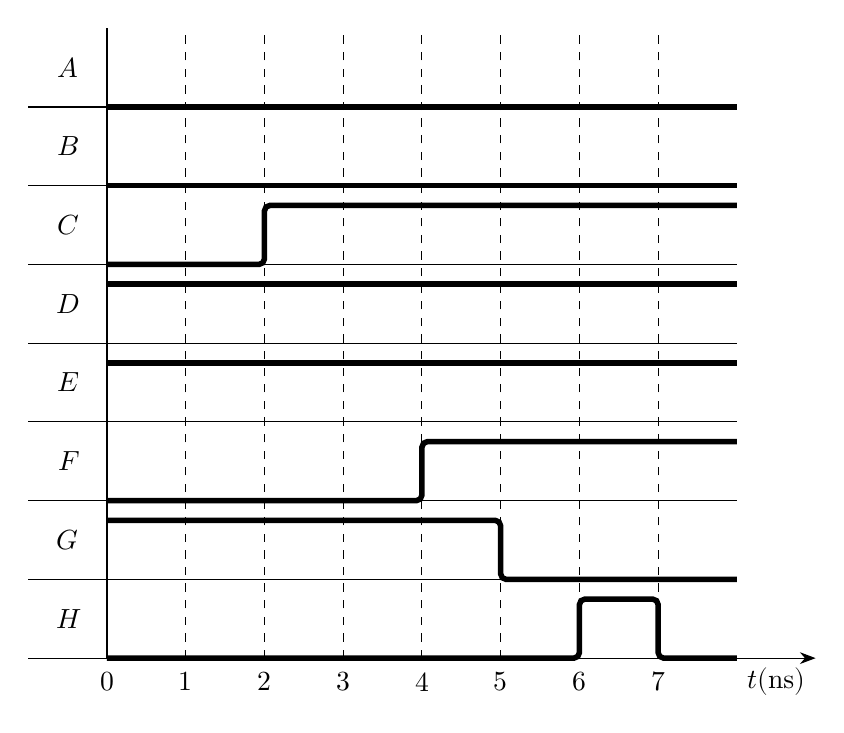
\begin{tikzpicture}[>={Stealth[length=2mm]}] 
\def\lshift{-0.3}    % yshift of label on axies
\def\rlimit{8}       % max x can time line reach
\def\hlevel{0.75}    % yshift of high level signal
% variables
\foreach \label [count=\cnt] in {H,...,A} {%
\node at (-0.5,\cnt-0.5) {$\label$}; \draw (-1,\cnt-1) --++ (\rlimit+1,0); 
};
% axies
\draw (0,0)--(0,8); \draw[->] (0,0)--(\rlimit+1,0);
\node at (0,\lshift) {0}; \node at (\rlimit+0.5,\lshift) {$t(\mathrm{ns})$};
% verticle lines
\foreach \x in {1,...,7} {%
\pgfmathtruncatemacro{\label}{\x}
\node at (\x,\lshift) {$\label$};
\draw[dashed] (\x,0) -- ++ (0,\rlimit);
};
% time line
\begin{scope}[line width=2pt,rounded corners=2pt]
\draw (0,7)--(\rlimit,7); % A
\draw (0,6)--(\rlimit,6); % B
\draw (0,5)--++(2,0)|-(\rlimit,5+\hlevel); % C
\draw (0,4+\hlevel)--(\rlimit,4+\hlevel); % D
\draw (0,3+\hlevel)--(\rlimit,3+\hlevel); % E
\draw (0,2)--++(4,0)|-(\rlimit,2+\hlevel); % F
\draw (0,1+\hlevel)--++(5,0)|-(\rlimit,1); % G
\draw (0,0)--++(6,0)|-++(1,\hlevel)|-(\rlimit,0); % H
\end{scope}
\end{tikzpicture}
\end{center}
\end{LTXexample}


\paragraph{卡诺图}\hspace{1pt}

\begin{LTXexample}[style=customlatex]
\usepackage{karnaugh-map} % 导言区
\begin{center}
\begin{karnaugh-map}[4][4][1][$AB$][$CD$]
    \minterms{0,4,5,7,8,10,11,12,14}
    \terms{1}{$X$}
    \implicant{0}{8}
    \implicant{5}{7}
    \implicant{11}{10}
    \implicantedge{12}{8}{14}{10}
    \end{karnaugh-map}
\end{center}
\end{LTXexample}

\paragraph{自动机}\hspace{1pt}


\begin{LTXexample}[pos=t,style=customlatex,style=linewrap]
\usepackage{tikz}
\usetikzlibrary{arrows.meta,calc,graphs,positioning,quotes,shapes} % 导言区
\begin{center}
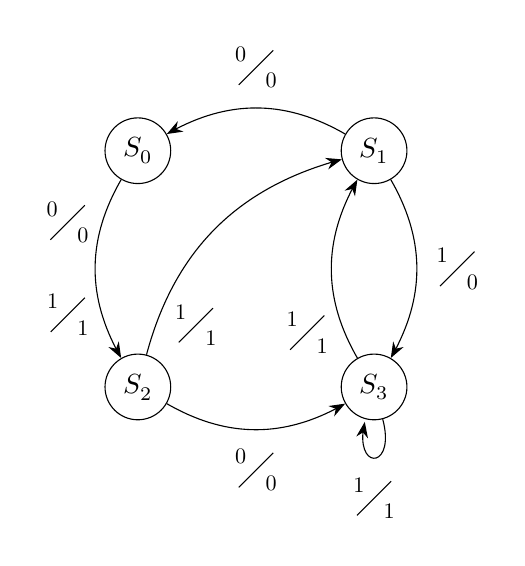
\begin{tikzpicture}[>={Stealth[length=2mm]}] 
\graph[math nodes, nodes={draw,circle}, edge quotes={auto,circle solidus,scale=0.8}, grow right=3cm, branch down=3cm] {
S_0 <- [bend left, "0 \nodepart{lower} 0"] S_1;
S_2 -> [bend right, "0 \nodepart{lower} 0" swap] S_3;
S_0 -> [bend right, "0 \nodepart{lower} 0" {swap,pos=0.4} ,"1 \nodepart{lower} 1" {swap,pos=0.6} ] S_2;
S_2 -> [bend left, "1 \nodepart{lower} 1" {swap,pos=0.2}] S_1;
S_3 -> [bend left, "1 \nodepart{lower} 1" pos=0.3] S_1;
S_1 -> [bend left, "1 \nodepart{lower} 0"] S_3;
S_3 -> [loop below, "1 \nodepart{lower} 1"] S_3;
};
\end{tikzpicture}
\end{center}
\end{LTXexample}


\paragraph{隐含表}\tagMACRO

\texttt{\bfseries implicantion}环境可以用于绘制隐含表,其定义和示例如下:

% Implication Table environment
% #1 cell size
\makeatletter
\newcounter{impt@@netcount}%
\newcounter{impt@@linecount}[impt@@netcount]%
\newcounter{impt@@columncount}[impt@@linecount]%
\newenvironment{implication}[1][1.5]{%
    \stepcounter{impt@@netcount}%
    \pgfmathsetmacro\cellsize{#1}%
    \pgfmathsetlengthmacro\cellsizelength{#1 cm}%
    % \drawcell{label}
    % draw a cell
    \newcommand*\impt@defcxy{%
        \pgfmathsetmacro\cx{\cellsize*\arabic{impt@@columncount}}%
        \pgfmathsetmacro\cy{-\cellsize*\arabic{impt@@linecount}}%
    }
    \newcommand*\impt@putnode[1]{%
        \node [draw,minimum size=\cellsizelength,align=center] at (\cx,\cy) {##1};%
        \stepcounter{impt@@columncount}%
        \ifnum\the\value{impt@@columncount}>\the\value{impt@@linecount}%
            \stepcounter{impt@@linecount}%
        \fi%
    }
    \newcommand*\impt@putx{%
        \draw ({\cx-0.3*\cellsize},{\cy-0.3*\cellsize})--++(0.6*\cellsize,0.6*\cellsize);%
        \draw ({\cx-0.3*\cellsize},{\cy+0.3*\cellsize})--++(0.6*\cellsize,-0.6*\cellsize);
    }
    \newcommand*\drawcell@star[1]{%
        \impt@defcxy%
        \impt@putnode{##1}%
    }
    \newcommand*\drawcell@nostar[1]{%
        \impt@defcxy%
        \impt@putnode{##1}%
        \impt@putx%
    }
    \newcommand*\drawcell{%
        \@ifstar{\drawcell@star}{\drawcell@nostar}%
    }
    % \drawlabelv{labels}
    % draw vertical labels
    \newcommand*\drawlabelv[1]{%
        \foreach \label [count=\n from 0] in {##1}{%
            \node [anchor=east] at ({-\cellsize*0.5},{-\cellsize*\n}) {\label};%
        }%
    }
    % \drawlabelh{labels}
    % draw horizontal labels
    \newcommand*\drawlabelh[1]{%
        \foreach \label [count=\n from 0] in {##1}{%
            \node [anchor=north] at ({\cellsize*\n},{-\cellsize*(\arabic{impt@@linecount}-0.5)}) {\label};%
        }%
    }
}{}
\makeatother

\lstinputlisting[frame=single,style=customlatex,style=linewrap]{implication.tex}

\begin{LTXexample}[varwidth,style=customlatex,style=linewrap]
\usepackage{tikz} % 导言区
\begin{center}
\begin{tikzpicture}
\begin{implication}[1.35]
%S_1
\drawcell*{$b-g$}
%c
\drawcell{$b-g$\\$c-f$}
\drawcell{$c-f$}
%d
\drawcell{}
\drawcell{} 
\drawcell{}
%e
\drawcell{$b-d$\\$e-f$}
\drawcell{$d-g$\\$e-f$}
\drawcell*{$c-e$\\$d-g$}
\drawcell{}
%f
\drawcell*{$a-f$}
\drawcell{$a-f$\\$b-g$}
\drawcell{$a-c$\\$b-g$}
\drawcell{}
\drawcell{$a-e$\\$b-d$}
%g
\drawcell{}
\drawcell{}
\drawcell{}
\drawcell*{$a-f$}
\drawcell{}
\drawcell{}
%labels
\drawlabelv{$b$,$c$,$d$,$e$,$f$,$g$}
\drawlabelh{$a$,$b$,$c$,$d$,$e$,$f$}
\end{implication}
\end{tikzpicture}
\end{center}
\end{LTXexample}

\subsubsection{程序设计}

\paragraph{流程图}\hspace{1pt}

\begin{LTXexample}[varwidth,style=customlatex,style=linewrap]
\usepackage{tikz}
\usetikzlibrary{arrows.meta,graphs,quotes}
\usepackage{flowchart}
% 导言区
\begin{center}
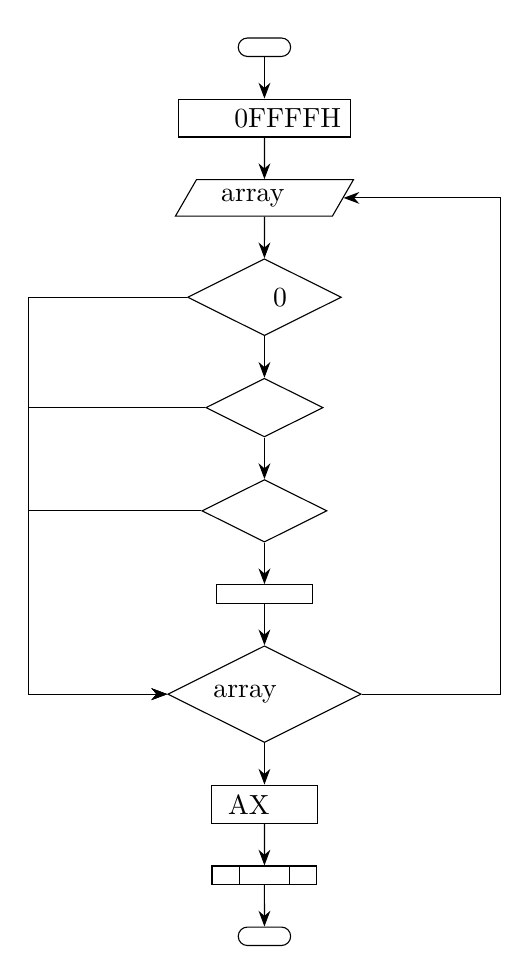
\begin{tikzpicture}[
>={Stealth[length=2mm]},
io/.style = {draw, trapezium, trapezium left angle=60, trapezium right angle=120},
decide/.style={draw, diamond, shape aspect=#1},
decide/.default={2},
term/.style = {draw, terminal},
proc/.style = {draw, process},
preproc/.style = {draw, predproc},
hv path/.style = 
{to path={-| (\tikztotarget) \tikztonodes}},
vh path/.style = 
{to path={|- (\tikztotarget) \tikztonodes}},
skip loop/.style = 
{to path={-- ++(0,#1) \tikztonodes -| (\tikztotarget) }},
vskip loop/.style = 
{to path={-- ++(#1,0) \tikztonodes |- (\tikztotarget) }},
every to quotes/.style={auto, near start},
every edge quotes/.style={auto, near start}
]
\graph[grow down sep=1.5em]
{ 
s [term,as=开始]->
a [proc,as=将答案赋值为0FFFFH]->
b [io,as=读入array的下一个数]->
c [decide,as=读入的数为0?]->["否"]
d [decide,as=读入的数为奇数?]->["否"]
e [decide,as=读入的数小于答案?]->["否"]
f [proc,as=将答案赋值为读入的数]->
g [decide,as=array读取完毕?]->["是"]
h [proc,as=将AX赋值为答案]->
i [preproc,as=打印答案]->
t [term,as=结束];
c ->["是", vskip loop=-3cm] g;
d ->["是", vskip loop=-3cm] g;
e ->["是", vskip loop=-3cm] g;
g ->["否", vskip loop=3cm] b;
};
\end{tikzpicture}
\end{center}
\end{LTXexample}
    
\subsubsection{操作系统}

\paragraph{调度结果图}\hspace{1pt}

\texttt{\bfseries dispatchgraph}环境可以用于绘制隐含表,其定义和示例如下:

\newcommand*\dgset[1]{%
\pgfkeys{%
/dispatch graph/.cd,#1%
}}
\dgset{
    xscale/.initial = 1,
    height/.initial = 1,
    fill/.initial = yellow!20
}
\newenvironment{dispatchgraph}
{%
    \newcommand*\dgcalc{%
        \edef\dgheight{\pgfkeysvalueof{/dispatch graph/height}}%
        \edef\dgxscale{\pgfkeysvalueof{/dispatch graph/xscale}}%
    }
    \newcommand*\drawdgmark[1][0]{%
        \dgcalc%
        \draw ({##1 * \dgxscale}, -0.5) -- ({##1 * \dgxscale}, \dgheight);%
        \node at ({##1 * \dgxscale}, -0.75) {##1};%
    }
    \newcommand*\drawslice[2]{%
        \dgcalc%
        \filldraw[fill=\pgfkeysvalueof{/dispatch graph/fill}] ({\dgxcur * \dgxscale}, 0) -| ({##1 * \dgxscale}, \dgheight) -| cycle;%
        \node at ({(\dgxcur + ##1) * \dgxscale * 0.5}, {\dgheight * 0.5}) {##2};%
        \drawdgmark[##1]
        \pgfmathsetmacro\dgxcur{##1}%
    }
    \begin{tikzpicture}%
    \pgfmathsetmacro\dgxcur{0}%
    \drawdgmark[0]%
}{%
    \end{tikzpicture}%
}

\lstinputlisting[frame=single,style=customlatex,style=linewrap]{dispatchgraph.tex}

\begin{LTXexample}[pos=t,style=customlatex,style=linewrap]
\usepackage{tikz} 
\dgset{
    height = 2,
    xscale = 0.25,
    fill = yellow
} % 导言区
\begin{center}
\begin{dispatchgraph}
    \drawslice{15}{$P_1$}
    \drawslice{35}{$P_2$}
    \drawslice{43}{$P_3$}
    \drawslice{55}{$P_4$}
    \drawslice{60}{$P_5$}
\end{dispatchgraph}
\end{center}
\end{LTXexample}
\end{document}